% =========================================================================
%  Finite Prevention Windows for HIV Post-Exposure Prophylaxis:
%  Irreversible Proviral Integration Defines Route-Specific Intervention Limits
%
%  A.C. Demidont, Nyx Dynamics LLC
%
%  Manuscript v2 prepared for Science Advances (manuscript ID aeh5879).
%  v2 incorporates self-disclosed methodological corrections and
%  reproducibility refinements from the 2026-04-30 disclosure tag.
%
%  Compile with:  pdflatex main_v2 && pdflatex main_v2 && pdflatex main_v2
% =========================================================================
\documentclass[11pt]{article}

% ---- Encoding & fonts ---------------------------------------------------
\usepackage[T1]{fontenc}
\usepackage[utf8]{inputenc}
\usepackage{mathptmx}                 % Times-like roman + math
\usepackage[scaled]{helvet}           % Helvetica for sans
\usepackage{textcomp}

% ---- Page geometry (Science Advances manuscript ~ 1in margins) ---------
\usepackage[letterpaper,margin=1in]{geometry}
\usepackage{setspace}
\onehalfspacing

% ---- Math ---------------------------------------------------------------
\usepackage{amsmath,amssymb,amsthm}
\usepackage{bm}
\usepackage{mathtools}

% ---- Floats, tables, figures -------------------------------------------
\usepackage{graphicx}
\usepackage{booktabs}
\usepackage{array}
\usepackage{tabularx}
\usepackage{caption}
\usepackage[font=small,labelfont=bf]{caption}
\usepackage{float}

% ---- Lists, links, color -----------------------------------------------
\usepackage{enumitem}
\usepackage{xcolor}
\usepackage[colorlinks=true,linkcolor=black,citecolor=black,urlcolor=blue]{hyperref}

% ---- Bibliography (numbered, italic superscript -- Science style) ------
\usepackage[numbers,super,sort&compress,round]{natbib}
\renewcommand\citenumfont[1]{\textit{#1}}
\renewcommand{\bibnumfmt}[1]{\textit{#1}.}

% ---- Theorem environments ----------------------------------------------
\newtheorem{theorem}{Theorem}
\newtheorem{lemma}{Lemma}
\newtheorem{proposition}{Proposition}
\newtheorem{corollary}{Corollary}
\theoremstyle{definition}
\newtheorem{definition}{Definition}
\newtheorem{assumption}{Assumption}
\theoremstyle{remark}
\newtheorem*{remark}{Remark}

% ---- Convenience macros -------------------------------------------------
\newcommand{\Tseed}{T_{\text{seed}}}
\newcommand{\Tint}{T_{\text{int}}}
\newcommand{\Pseed}{P_{\text{seed}}}
\newcommand{\Pint}{P_{\text{int}}}
\newcommand{\Epep}{E_{\text{PEP}}}
\newcommand{\Ebarpep}{\bar{E}_{\text{PEP}}}
\newcommand{\Faccess}{F_{\text{access}}}
\newcommand{\tcrit}{t_{\text{crit}}}
\newcommand{\emax}{\varepsilon_{\max}}
\newcommand{\emid}{\varepsilon_{\text{mid}}}
\newcommand{\emin}{\varepsilon_{\min}}
\newcommand{\R}{\mathbb{R}}

% ---- Paragraph spacing --------------------------------------------------
\setlength{\parskip}{0.4em}
\setlength{\parindent}{0pt}

% ---- Section title formatting ------------------------------------------
\usepackage{titlesec}
\titleformat*{\section}{\large\bfseries}
\titleformat*{\subsection}{\normalsize\bfseries}

% =========================================================================
\begin{document}

% ---- Title block --------------------------------------------------------
\begin{flushleft}
{\LARGE\bfseries Finite Prevention Windows for HIV Post-Exposure Prophylaxis:\\[0.3em]
Irreversible Proviral Integration Defines Route-Specific Intervention Limits\par}
\vspace{1em}

{\large A.C. Demidont\textsuperscript{*}\par}
\vspace{0.5em}
\textit{Nyx Dynamics LLC, Philadelphia, PA 19107, USA}\\[0.3em]
\textsuperscript{*}Correspondence: \texttt{ac.demidont@nyxdynamics.com} \\
ORCID: 0000-0002-9216-8569
\end{flushleft}

\vspace{1em}

% ---- One-sentence summary (Science Advances requirement) ---------------
\noindent\textbf{One-sentence summary:} Irreversible proviral integration defines a finite prevention window that structural barriers systematically eliminate for people who inject drugs.

\vspace{1em}

% ---- Abstract -----------------------------------------------------------
\noindent\textbf{Abstract.}\quad
Proviral integration --- the molecular event that converts HIV infection from reversible to permanent --- defines a finite window during which post-exposure prophylaxis (PEP) can succeed. Using a multiscale within-host model that combines stochastic founder-phase tau-leaping with a deterministic ODE handoff and an eclipse-phase fixed delay anchored on Perelson 1996 ($\sim$22~h), we prove that PEP efficacy decays monotonically to zero and derive the critical prevention window from emergent integration kinetics rather than drug potency or hand-set parameters. This window is approximately 1.75-fold shorter for parenteral (injection) than mucosal (sexual) exposure, yielding a parenteral $\tcrit$ at $\eta = 0.05$ of approximately 34.5~hours ($V_{0} = 10^{3}$, CV$=0.3$) versus 60.5~hours mucosally ($V_{0} = 1$, CV$=0.3$) --- concordant with the empirical 1.5--2$\times$ compression range spanning Tsai 1998 (intravenous SIV) and Otten 2000 (intravaginal SHIV) NHP challenge data. Independent cascade-based modeling of structural access for people who inject drugs produces population-level prevention success of 0.003--0.7\% under current US policy [companion analysis], with a 92.7\% national 10-year outbreak probability. The analytical $\Faccess \times \tcrit$ upper bound ($\sim$11\%) is consistent with these point estimates as a conservative envelope. The failure mode is structural rather than pharmacological: PEP retains high per-exposure efficacy; population-level efficacy is bounded by the mismatch between access timing and integration timing.

\vspace{1em}
\hrule
\vspace{1em}

% =========================================================================
\section*{Introduction}

Retroviral infection is unique among infectious diseases in that a single molecular event --- proviral integration into the host genome --- converts a reversible inflammatory process into a permanent genomic state. This irreversibility is absolute: no antiviral intervention operating after integration can restore the pre-infection state. Post-exposure prophylaxis (PEP) exploits the finite interval before this transition, but the boundaries of that interval have never been formally derived from within-host kinetics. Here we prove, using a three-state absorbing Markov framework parameterized on established HIV-1 viral dynamics\cite{tanner2025,chun1995,siliciano2005}, that the prevention window is not a clinical convention but a mathematically necessary consequence of integration kinetics --- that it is route-specific, compressible by viral load, and in the case of parenteral (injection) exposure, potentially shorter than the structural delays that define healthcare access for people who inject drugs (PWID). The result transforms PEP timing from an empirical guideline into a derived biological quantity, and reveals that the 72-hour standard --- mechanistically appropriate for mucosal exposure --- cannot be assumed to generalize across routes or populations.

HIV-1 infection establishment involves two irreversible transitions whose timing governs the prevention window. First, free virus establishes a self-sustaining replicative focus (\emph{seeding}, time $\Tseed$). Second, infected cells commit stably integrated proviral DNA into long-lived reservoir cells (\emph{integration}, time $\Tint$). Once integration is complete, the cellular state is absorbing: no biologically realizable intervention restores the uninfected state, because integrated provirus is propagated to all daughter cells via clonal expansion\cite{chun1995,siliciano2005} and persists through ART, which suppresses replication but leaves the reservoir intact\cite{perelson1997}. This biological fact constrains PEP efficacy independently of drug potency.

% =========================================================================
\section*{Mathematical framework}

We model within-host state as a random variable $Z(t) \in \{0, 1, 2\}$, where $Z=0$ (susceptible), $Z=1$ (seeded, pre-integration), and $Z=2$ (integrated, absorbing). Transition times $\Tseed \leq \Tint$ are stopping times on the natural filtration of the exposure process. Under stage-dependent drug efficacy $\varepsilon(Z)$ --- with $\emax$ pre-seeding, $\emid$ post-seeding/pre-integration, and $\emin = 0$ post-integration --- the expected PEP efficacy at time $t$ is, by the law of total probability:
\begin{equation}
\Epep(t) = \big(1 - \Pseed(t)\big)\emax + \big(\Pseed(t) - \Pint(t)\big)\emid + \Pint(t)\,\emin
\label{eq:master}
\end{equation}
where $\Pseed(t) = \Pr(\Tseed \leq t)$ and $\Pint(t) = \Pr(\Tint \leq t)$. Since both cumulative probabilities are non-decreasing in $t$ and $\Pint(t) \to 1$, this yields the \textbf{Finite Prevention Window Theorem}: (i) $\Epep(t)$ is non-increasing; (ii) $\Epep(t) \to 0$; and (iii) for any threshold $\eta \in (0,1)$, there exists a finite critical time $\tcrit(\eta) = \inf\{t : \Epep(t) < \eta\}$, beyond which efficacy cannot be recovered regardless of drug potency. The rate of efficacy decay decomposes as
\begin{equation}
\frac{d\Epep}{dt} = -f_{\text{seed}}(t)\,\Delta\varepsilon_{1} - f_{\text{int}}(t)\,\Delta\varepsilon_{2} \;\leq\; 0
\label{eq:hazard}
\end{equation}
where $f_{\text{seed}}$ and $f_{\text{int}}$ are the transition probability densities and $\Delta\varepsilon_{1}, \Delta\varepsilon_{2}$ are the efficacy drops across transitions (Supplementary Text, Section~S4). The absorbing-state claim (Assumption~A1) is grounded in the standard target-cell-limited ODE system\cite{perelson1996}: under ART-induced suppression $I \to 0$, reservoir dynamics give $dR/dt = \alpha I \to 0$, so $R$ is constant --- the reservoir neither grows nor is cleared. This is the mathematical statement that ART controls but cannot eradicate HIV.

\textbf{Assumption: transmission-competent exposure.} The Finite Windows framework models within-host integration kinetics conditional on exposure to viremic source virus. We assume throughout that source plasma viral load is at or above the established U=U threshold ($\geq 200$~copies/mL sustained). The framework's predictions --- $\tcrit$, $\Faccess$, and the population-level efficacy bound --- are not applicable to exposures from virologically suppressed sources, for whom transmission risk is functionally zero\cite{rodger2019,bavinton2018}. U=U exposures are operationally outside scope: no PEP need arises.

% =========================================================================
\section*{Route-dependent window compression}

Parenteral inoculation differs from mucosal exposure in its initial condition: direct intravascular delivery bypasses epithelial barriers, producing a substantially larger effective inoculum. We model mucosal exposure as $V^{(m)}(0) = 1$ virion/mL (post-epithelial attenuation) versus parenteral $V^{(p)}(0) = 10^{3}$ virions/mL. By monotone systems theory applied to the target-cell-limited ODE (Lemma~S5.2), larger initial inoculum produces earlier $I(t)$ and consequently earlier $R(t)$ accumulation, yielding first-order stochastic dominance: $\Pint^{(p)}(t) \geq \Pint^{(m)}(t)$ for all $t$. It follows directly that $\Epep^{(p)}(t) \leq \Epep^{(m)}(t)$ and $\tcrit^{(p)}(\eta) \leq \tcrit^{(m)}(\eta)$ for any threshold $\eta$ (Corollary~S5.1).

% =========================================================================
\section*{Multiscale model and parameterization}

The framework is implemented as a two-phase multiscale within-host model. \textbf{Phase~1} simulates founder-population dynamics stochastically via tau-leaping at low inoculum ($V_{0} \leq I_{\text{handoff}} = 10$), capturing extinction events for sparse founder populations. \textbf{Phase~2} integrates the deterministic target-cell-limited ODE system once productive infection is established, anchored on the within-host kinetic literature: viral clearance rate $c = 23$~day$^{-1}$ (virion $t_{1/2} \approx 0.7$~h; Ramratnam et al.\ 1999\cite{ramratnam1999}, refining the earlier Perelson 1996\cite{perelson1996} estimate), infected-cell death rate $\delta = 0.7$~day$^{-1}$\cite{perelson1996}, eclipse phase $\tau = 0.9$~days ($\approx 22$~h; Perelson 1996, Table~2). Standard within-host parameters\cite{mcmichael2010}: target cell production $\lambda = 10^{4}$~cells/mL/day, natural death $d_{T} = 0.01$~day$^{-1}$, infection rate $\beta = 2.4 \times 10^{-5}$~mL$\cdot$virion$^{-1}\cdot$day$^{-1}$, viral production $p = 10^{3}$~virions/cell/day, integration rate $\alpha = 10^{-3}$~day$^{-1}$. Heterogeneity is implemented as multiplicative log-normal variation (CV $= 0.3$) on $\{\beta, c, \delta, \alpha\}$. The eclipse phase is implemented as a discrete fixed-delay buffer between cell infection and integration competence, ensuring that the lower bound on $\Tint$ is the biological eclipse floor. We use $N = 500$ realizations per (route, $V_{0}$, CV) cell across the parameter sweep; the canonical operating point is parenteral $V_{0} = 10^{3}$ at CV $= 0.3$ and mucosal $V_{0} = 1$ at CV $= 0.3$. Drug efficacy parameters: $\emax = 0.95$, $\emid = 0.50$, $\emin = 0$. Integration time $\Tint$ is the first time $R(t) \geq R^{*} = 10$~cells/mL. Threshold sensitivity ($I^{*} \in [10, 1000]$, $R^{*} \in [1, 100]$) shifts $\tcrit^{(p)}$ by $<8$~h and maintains the qualitative compression result.

% =========================================================================
\section*{Results: route-specific windows}

Figure~\ref{fig:route} shows the predicted $\Epep(t)$ curves for both routes derived from the multiscale model at the cited submission SHA. The mucosal window $\tcrit^{(m)}(0.05) \approx 60.5$~hours at $V_{0} = 1$ (CV $= 0.3$) emerges from within-host kinetics and falls within the operational 72-hour CDC mucosal-PEP guideline\cite{tanner2025}, providing mechanistic context for the clinical threshold. The parenteral window compresses to $\tcrit^{(p)}(0.05) \approx 34.5$~hours at $V_{0} = 10^{3}$ (CV $= 0.3$) --- a $\approx$1.75-fold reduction. The route compression ratio is concordant with the empirical NHP range of 1.5--2$\times$ spanning Tsai et al.\cite{tsai1995} (intravenous SIV: complete protection at 24~h, 50\% at 48~h) and Otten et al.\cite{otten2000} (intravaginal SHIV: complete protection through 36~h, 50\% at 72~h). At the within-host kinetic level, the model captures full protection at early delays (Otten 12~h, 36~h: model $\Epep = 0.95$ vs.\ NHP 1.00) but under-predicts protection at later timepoints (Tsai 24~h, 48~h; Otten 72~h). We interpret this gap as evidence of NHP-specific protective contributions not captured by the within-host kinetic framework alone --- an empirical limit of the model's domain rather than a refutation of the compression result. Table~\ref{tab:nhp} summarizes per-timepoint concordance.

% =========================================================================
\section*{Stochastic efficacy analysis}

Monte Carlo integration of Equation~\ref{eq:master} over source viral load (VL) distributions (Fig.~\ref{fig:stochastic}A--B) reveals three empirically distinct temporal regimes defined by the 95\% credible-interval (CI) width of the stochastic efficacy distribution. \textit{Regime~1} (0--22~h): CI is narrow ($<$15 percentage points) and efficacy is high ($>$90\% mean for PWID-relevant VL distributions); VL knowledge adds limited decision-relevant precision. \textit{Regime~2} (22--78~h for PWID/acute; 22--88~h for mixed/general distributions): CI width is maximal, peaking at 39.7~percentage points at 49~h for untreated PWID VL distributions (mean $\log_{10} = 4.5$, SD $= 1.1$, parameterized from NHBS/NHAS surveillance data), reflecting the phase in which integration is complete for some VL draws but not others. \textit{Regime~3} ($>$78~h): CI collapses as efficacy converges to zero across all VL draws. The regime transition at $\approx$22~h is mechanistically interpretable: it corresponds to the eclipse phase lower bound from Perelson et al.\cite{perelson1996} ($\approx 0.9$~days $\approx$ 22~h), below which integration cannot yet be complete for any draw. Threshold probability analysis shows that $P(\text{efficacy} < 50\%) = 100\%$ across all distributions at 48~h and that $P(\text{futile})$ --- defined as $P(\text{efficacy} < 5\%)$ --- reaches 91.8\% (PWID untreated) and 98.8\% (acute-infection-enriched network) by 72~h (Table~\ref{tab:stochastic}).

% =========================================================================
\section*{City-stratified analysis}

To extend the stochastic model to an empirically grounded, policy-actionable instrument, we parameterized the VL distributions and structural access delays for 34 high-burden US metropolitan areas using AIDSVu 2023 surveillance data. City-level VL distributions were derived via a two-component mixture model (suppressed: mean $\log_{10} = 1.5$, SD $= 0.4$; unsuppressed: mean $\log_{10} = 4.5$, SD $= 1.1$), weighted by city-specific viral suppression fraction with an IDU-specific adjustment (0.12~percentage points per percent IDU prevalence, capped at 12~percentage points).

\subsection*{City-level structural delay (population-level access friction)}

Structural access delay was estimated from AIDSVu late-diagnosis and linkage-to-care percentages as
\begin{equation}
\Delta t_{\text{structural}} = \beta_{1}\,(\text{LateDx}\% - 10\%) + \beta_{2}\,\max(90\% - \text{Linkage}\%,\, 0) + \Delta t_{\text{SDOH}}
\label{eq:delay}
\end{equation}
with coefficients $\beta_{1} = 1.2$~h/\% and $\beta_{2} = 0.3$~h/\% calibrated to yield $\approx$6~hours at the median city. City-level structural delay is operationalized as a composite indicator combining AIDSVu late-diagnosis percentage and linkage-to-care percentage according to the functional form specified in Equation~\ref{eq:delay}. The composite is a constructed measure of healthcare access friction; it is not a proxy under proximal causal inference\cite{tchetgentchetgen2020}, and the analysis does not invoke the identification conditions required for proxy-based estimation\cite{pearl2009}. The distinction matters because related work in this research program does invoke proxy-based identification under those conditions.

Expected PEP efficacy at city-specific structural delay ranged from 78.8\% (Hartford CT; structural delay 24.4~h; IDU prevalence 23.4\%) to 98.3\% (Milwaukee WI; 1.9~h), a 19.5~percentage-point spread correlated almost entirely with structural delay rather than community VL (Pearson $r = -0.935$ vs.\ $-0.084$, respectively; Fig.~\ref{fig:city}). Cities with high IDU prevalence exhibit consistently longer structural delays and lower viral suppression simultaneously, narrowing the PEP window from both directions at once.

% =========================================================================
\section*{Population-level efficacy: three independent lines of evidence}

\subsection*{(a) Cascade-based point estimates}

Companion modeling\cite{demidont_companion} applies an architectural barrier framework ($n = 100{,}000$ PWID, 5-year horizon) and an independent PWID Monte Carlo simulation to compute the probability that an individual PWID achieves the full prevention cascade ($P(R_{0}=0)$) under structural conditions. Under current US policy: the architectural-barrier model produces $P(R_{0}=0) = 0.003\%$ [95\% CI 0.000--0.006\%]; the independent PWID simulation produces $0.007\%$. Decriminalization-only intervention raises this to 0.198--0.814\%; full harm reduction raises it to 9.55\%. The same architectural model applied to MSM under identical structural assumptions produces $16.3\%$ prevention success --- a $\approx$5{,}400-fold population-level disparity between routes.

\subsection*{(b) Outbreak probability forecasting}

Independent stochastic outbreak modeling\cite{demidont_companion} forecasts a $73.8\%$ probability of major HIV outbreak among PWID nationally within 5 years under current policy (95\% PSA CI 63.5--82.0\%) and $92.7\%$ within 10 years; regional probabilities reach $86.3\%$ (Pacific Northwest) and $78.4\%$ (Appalachia) within 5 years. Median time-to-outbreak is 3 years.

\subsection*{(c) Analytical $\Faccess \times \tcrit$ envelope (this paper) --- individual-level access distribution}

The timing mismatch can be formalized as a distribution-free inequality. For access delay distribution $\Faccess$, the expected population-level PEP efficacy satisfies
\begin{equation}
\Ebarpep \;\leq\; \Faccess(\tcrit^{(p)})\,\emax + \big(1 - \Faccess(\tcrit^{(p)})\big)\,\eta
\label{eq:bound}
\end{equation}
(Proposition~S6.1). The bound requires only the fraction of the population accessing PEP within the parenteral window --- not the full parametric form of $\Faccess$. Modeling access delay as log-normal (median 96~h, geometric SD 2.0; modeling choice informed by qualitative discussion in the PWID PEP-access literature\cite{taylor2019,baugher2025}; the specific median is a defensible parameterization rather than an empirical anchor lifted from primary timing data) yields $\Faccess(34.5~\text{h}) \approx 0.070$. With $\eta = 0.05$ and $\emax = 0.95$, Equation~\ref{eq:bound} yields $\Ebarpep \leq 0.070 \times 0.95 + 0.930 \times 0.05 \approx 11.3\%$ --- the most generous (envelope) reading of population-level PEP efficacy. Sensitivity analysis across plausible median values $F_{\text{median}} \in \{72, 96, 110, 120\}$~hours yields envelope estimates of 7.5\%--15.9\% (Table~\ref{tab:bound}); in all cases, the envelope is one to four orders of magnitude above the cascade point estimates in (a) and is consistent with the outbreak probabilities in (b) as a conservative upper bound.

\subsection*{Convergent finding}

Three independent modeling approaches --- cascade-based individual-level prevention probability, system-level outbreak forecasting, and analytical $\Faccess \times \tcrit$ envelope --- all support the conclusion that PEP cannot serve as a population-level safety net for PWID under current structural conditions. The analytical envelope is the least favorable estimate; the cascade-based central estimates are 100--3{,}000$\times$ more pessimistic and remain qualitatively consistent.

\subsection*{Limitation: $\Faccess$ denominator}

$\Faccess$ here is derived from population-wide PEP-access surveillance, which includes exposures from both transmission-competent and virologically suppressed sources. Under U=U\cite{rodger2019,bavinton2018}, exposures from suppressed sources have functionally zero transmission risk and are outside the framework's domain. Restricting $\Faccess$ to transmission-competent exposures only would reduce the relevant denominator and yield a tighter (smaller) $\Faccess$ and a tighter bound. This refinement strengthens, rather than weakens, the conclusion.

% =========================================================================
\section*{Stochastic VL uncertainty and the critical window}

The source VL knowledge premium --- the gain from knowing source VL precisely versus marginalizing over the distribution --- peaks at 2.9~percentage points at 21~h for PWID untreated and 3.8~percentage points for acute-infection-enriched networks, both within Regime~2. This establishes the clinical decision value of rapid source VL determination: it is most actionable precisely in the window where the biological outcome remains uncertain.

% =========================================================================
\section*{Implications}

Two conclusions follow. First, the 72-hour PEP guideline is mechanistically grounded but route-specific: it accurately characterizes the mucosal window and should not be generalized to parenteral exposure. The parenteral window is shorter by a factor determined by within-host kinetics, and that factor is concordant with NHP empirical data. Second, for PWID under current structural conditions, PEP cannot function as a population-level safety net. Since PEP and pre-exposure prophylaxis (PrEP) are the only two biomedical prophylaxis modalities for HIV\cite{grant2010,anderson2012}, and PrEP uptake among PWID remains below 1\% of those with indication\cite{baugher2025}, this population effectively lacks both options. Long-acting injectable PrEP, demonstrated to provide effective pre-exposure protection against parenteral challenge in NHP studies\cite{swanstrom2023,vidal2022}, is the modality most capable of bridging this gap --- if structural delivery barriers are addressed\cite{demidont2026}. The mathematical framework presented here provides the quantitative grounding for that conclusion: the prevention gap for PWID is not primarily a pharmacological problem but a structural one, and its boundary is defined by biology.

All efficacy and access estimates herein are conditional on a transmission-competent exposure; the framework does not apply to U=U exposures (source viral load $<200$~copies/mL sustained), for whom transmission risk is functionally zero, and the policy implications drawn here pertain only to populations with non-suppressed source viremia.

% =========================================================================
\section*{Conclusion}

PEP is not the safety net for parenteral HIV exposure that it is for sexual transmission. We prove that proviral integration establishes a finite, route-specific prevention window; that this window is approximately 1.75-fold shorter for parenteral than for mucosal exposure; and that structural access delays for PWID systematically consume this window. Across three independent modeling approaches --- cascade-based prevention probability, system-level outbreak forecasting, and analytical $\Faccess \times \tcrit$ envelope --- population-level PEP efficacy for PWID under current structural conditions is bounded between approximately $0.003\%$ (cascade central estimate) and $11\%$ (analytical envelope), with corresponding $92.7\%$ 10-year outbreak probability under current policy. The conclusion is not a statement against PEP for individuals who present in time. It is a quantitative argument that pre-exposure prevention is the primary biomedical tool available for this population --- and that current deployment levels are insufficient to close the gap.

% =========================================================================
\section*{Materials and Methods}

\subsection*{Mathematical proofs}
All formal proofs (Theorem~1, Corollaries~1--2, Lemmas~1--2, Propositions~1--3) are provided in the Supplementary Text. The absorbing-state ODE system, hazard-rate decomposition, monotone systems comparison argument, and population-efficacy bound are each derived in full.

\subsection*{Software environment and reproducibility}
All computational analyses were performed in Python 3.11 with NumPy, SciPy, matplotlib, and pandas. Complete environment specifications, including pinned package versions, are provided in \texttt{requirements.txt} in the project repository. Monte Carlo simulations used fixed random seeds (\texttt{np.random.default\_rng(base\_seed*1{,}000{,}000+k)}) to ensure deterministic reproducibility from the cited commit (SHA \texttt{37e27ea}). Independent re-execution from the cloned repository at the cited SHA reproduces all numerical claims to full floating-point precision; this was verified prior to manuscript revision.

\subsection*{Numerical simulation}
The multiscale model (Phase~1 stochastic tau-leaping + Phase~2 deterministic ODE handoff + eclipse-phase fixed-delay buffer) was implemented in Python. Monte Carlo replicate count ($N = 500$ per (route, $V_{0}$, CV) cell; $\sim$27{,}000 realizations across the full parameter sweep) was selected to achieve standard error below 1~percentage point on cumulative integration probabilities at clinical timepoints (24~h, 48~h, 72~h). Sensitivity to $N$ at the canonical operating point ($V_{0} = 10^{3}$ parenteral, CV $= 0.3$) was tested at $N \in \{200, 500, 1000, 5000\}$; $\tcrit$ estimates stable to within $\pm 0.5$~h across this range. Integration time $\Tint$ was computed as the first time $R(t) \geq R^{*} = 10$~cells/mL. Efficacy curves were computed as in Equation~\ref{eq:master} with $\emax = 0.95$, $\emid = 0.50$, $\emin = 0$. Threshold sensitivity analysis varied $I^{*} \in [10, 1000]$~cells/mL and $R^{*} \in [1, 100]$~cells/mL across a $20 \times 20$ grid. Stochastic VL integration used 50 time points, 0--120~h, with 10{,}000 VL draws per time point.

\subsection*{Sex as a biological variable}
The within-host kinetic framework operates on cellular and viral dynamics that have not been established to differ by sex at the resolution of the available data; the foundational Perelson 1996 cohort\cite{perelson1996} was small (5 patients) and did not establish sex-specific kinetic parameters. The city-stratified analysis pools across sex within AIDSVu surveillance categories, which provide sex-stratified late-diagnosis and viral suppression data; sex-stratified replication of the city analysis is a defensible extension but is not pursued here as the structural-barrier conclusions are robust to within-stratum variation.

\subsection*{City-stratified parameterization}
City-level viral suppression, late-diagnosis, and linkage-to-care data were obtained from AIDSVu downloadable datasets for 34 high-burden US metropolitan areas (2023 reporting year). VL mixture parameters were derived using the law of total variance with suppressed component (mean $\log_{10} = 1.5$, SD $= 0.4$) and unsuppressed component (mean $\log_{10} = 4.5$, SD $= 1.1$). IDU suppression adjustment: 0.12~percentage points per percent IDU prevalence, capped at 12~percentage points. Structural delay coefficients calibrated to median city yield $\approx$6~hours. Counterfactual analysis assigned all cities a uniform 24-hour delay. Full dataset and derivation scripts are in the code repository.

% =========================================================================
% References (Science style: italic numbers)
% =========================================================================
\renewcommand{\refname}{\large\textbf{References and Notes}}

\begin{thebibliography}{99}

\bibitem{tanner2025}
M.R. Tanner \textit{et al.}, Antiretroviral postexposure prophylaxis after sexual, injection drug use, or other nonoccupational exposure to HIV --- CDC recommendations, United States, 2025. \textit{MMWR Recomm. Rep.} \textbf{74}(1), 1--56 (2025).

\bibitem{chun1995}
T.W. Chun, D. Finzi, J. Margolick, K. Chadwick, D. Schwartz, R.F. Siliciano, In vivo fate of HIV-1-infected T cells: quantitative analysis of the transition to stable latency. \textit{Nat. Med.} \textbf{1}, 1284--1290 (1995).

\bibitem{siliciano2005}
J.D. Siliciano, R.F. Siliciano, Enhanced culture assay for detection and quantitation of latently infected, resting CD4$^{+}$ T-cells carrying replication-competent virus in HIV-1-infected individuals, in \textit{Human Retrovirus Protocols} (Humana Press, New Jersey, 2005), vol.~304, pp.~3--16.

\bibitem{perelson1997}
A.S. Perelson \textit{et al.}, Decay characteristics of HIV-1-infected compartments during combination therapy. \textit{Nature} \textbf{387}, 188--191 (1997).

\bibitem{perelson1996}
A.S. Perelson, A.U. Neumann, M. Markowitz, J.M. Leonard, D.D. Ho, HIV-1 dynamics \textit{in vivo}: virion clearance rate, infected cell life-span, and viral generation time. \textit{Science} \textbf{271}, 1582--1586 (1996).

\bibitem{ramratnam1999}
B. Ramratnam \textit{et al.}, Rapid production and clearance of HIV-1 and hepatitis C virus assessed by large volume plasma apheresis. \textit{Lancet} \textbf{354}, 1782--1785 (1999). [Updated virion clearance rate $c \approx 23$~day$^{-1}$, $t_{1/2} \approx 0.7$~h, supplanting the Perelson 1996 estimate.]

\bibitem{mcmichael2010}
A.J. McMichael, P. Borrow, G.D. Tomaras, N. Goonetilleke, B.F. Haynes, The immune response during acute HIV-1 infection: clues for vaccine development. \textit{Nat. Rev. Immunol.} \textbf{10}, 11--23 (2010).

\bibitem{tsai1995}
C.C. Tsai \textit{et al.}, Prevention of SIV infection in macaques by (R)-9-(2-phosphonylmethoxypropyl)adenine. \textit{Science} \textbf{270}, 1197--1199 (1995). [Timing data: \textit{J. Virol.} \textbf{72}, 4265--4273 (1998)]

\bibitem{otten2000}
R.A. Otten, D.K. Smith, D.R. Adams, J.K. Pullium, E. Jackson, C.N. Kim, H. Jaffe, R. Janssen, S. Butera, T.M. Folks, Efficacy of postexposure prophylaxis after intravaginal exposure of pig-tailed macaques to a human-derived retrovirus (human immunodeficiency virus type 2). \textit{J. Virol.} \textbf{74}, 9771--9775 (2000).

\bibitem{rodger2019}
A.J. Rodger \textit{et al.}, Risk of HIV transmission through condomless sex in serodifferent gay couples with the HIV-positive partner taking suppressive antiretroviral therapy (PARTNER): final results of a multicentre, prospective, observational study. \textit{Lancet} \textbf{393}, 2428--2438 (2019).

\bibitem{bavinton2018}
B.R. Bavinton \textit{et al.}, Viral suppression and HIV transmission in serodiscordant male couples: an international, prospective, observational, cohort study (Opposites Attract). \textit{Lancet HIV} \textbf{5}, e438--e447 (2018).

\bibitem{taylor2019}
J.L. Taylor, A.Y. Walley, A.R. Bazzi, Stuck in the window with you: HIV exposure prophylaxis in the highest risk people who inject drugs. \textit{Subst.\ Abus.} \textbf{40}, 441--443 (2019). [Commentary; cited for qualitative discussion of structural barriers, not primary timing data.]

\bibitem{baugher2025}
A.R. Baugher \textit{et al.}, Are we ending the HIV epidemic among persons who inject drugs? Key findings from 19 US cities. \textit{AIDS} \textbf{39}(12), 1813--1819 (2025).

\bibitem{tchetgentchetgen2020}
E.J. Tchetgen Tchetgen, A. Ying, Y. Cui, X. Shi, W. Miao, An introduction to proximal causal inference. \textit{Statistical Science} \textbf{39}, 375--390 (2024). [Pre-print 2020; final published version 2024. Cite specifically for the formal definition of proxy variables under proximal causal inference.]

\bibitem{pearl2009}
J. Pearl, \textit{Causality: Models, Reasoning, and Inference}, 2nd ed.\ (Cambridge University Press, 2009).

\bibitem{grant2010}
R.M. Grant \textit{et al.}, Preexposure chemoprophylaxis for HIV prevention in men who have sex with men. \textit{N. Engl. J. Med.} \textbf{363}, 2587--2599 (2010).

\bibitem{anderson2012}
P.L. Anderson \textit{et al.}, Emtricitabine--tenofovir concentrations and pre-exposure prophylaxis efficacy. \textit{Sci. Transl. Med.} \textbf{4}, 151ra125 (2012).

\bibitem{swanstrom2023}
A.E. Swanstrom \textit{et al.}, Long-acting lenacapavir protects macaques against intravenous challenge with simian-tropic HIV. \textit{eBioMedicine} \textbf{95}, 104764 (2023).

\bibitem{vidal2022}
S.J. Vidal \textit{et al.}, Long-acting capsid inhibitor protects macaques from repeat SHIV challenges. \textit{Nature} \textbf{601}, 612--616 (2022).

\bibitem{demidont2026}
A.C. Demidont, Clinical decision support algorithm for LAI-PrEP bridge period navigation at UNAIDS global target scale. \textit{Viruses} (2026; accepted).

\bibitem{emau2006}
P. Emau \textit{et al.}, Post-exposure prophylaxis for SIV revisited: animal model for HIV prevention. \textit{AIDS Res.\ Ther.} \textbf{3}, 8 (2006).

\bibitem{demidont_companion}
A.C. Demidont, Structural barriers, stochastic avoidance, and outbreak risk in HIV prevention for people who inject drugs. \textit{[Companion manuscript; in preparation / preprint DOI to be assigned]}.

\end{thebibliography}

% =========================================================================
\vspace{1em}
\hrule
\vspace{0.5em}

\section*{Acknowledgments}
The author thanks the HIV prevention research community whose published work informed model parameterization, and PWID community advocates whose testimony informed characterization of structural barriers.

\textbf{Funding:} No external funding was received.

\textbf{Author contributions:} A.C.D.: conceptualization, formal analysis, mathematical proofs, simulation, writing.

\textbf{Competing interests:} The author reports prior employment with Gilead Sciences, Inc.\ from January 2020 through November 2024, and held company stock during that period; all Gilead stock was fully divested by December 2024. Employment ended prior to the initiation of this research. Gilead Sciences had no role in study conception, design, data collection, analysis, interpretation, writing, or the decision to submit for publication. The manuscript references lenacapavir, a Gilead product, as one member of the long-acting injectable antiretroviral class; the mathematical conclusions of this work are pharmacologically agnostic and pertain to the class as a whole. The author is the sole owner of Nyx Dynamics LLC, under whose affiliation this research was conducted independently.

\textbf{Data and materials availability:} Code and data are archived at Zenodo (DOI: \texttt{10.5281/zenodo.20044747}) under the GitHub release tagged for this submission. The repository (\url{https://github.com/Nyx-Dynamics/Prevention-Theorem} at commit \texttt{37e27ea}) separates source code (\texttt{SRC/}), simulation outputs (\texttt{results/}), and processed datasets (\texttt{data/}); a \texttt{README.md} at the repository root documents the file layout and reproduction sequence. The numerical claims in this paper --- including parenteral $\tcrit = 34.5$~h, mucosal $\tcrit = 60.5$~h, and the NHP concordance values --- reproduce from \texttt{SRC/multiscale\_model/run\_mc\_v3.py} at this SHA (verified 2026-05-05). A reconciled summary of all numerical claims with source files and commit references is provided as \texttt{numerical\_claims\_v2.csv} in the supplementary materials. No individual-level human data were used; all surveillance data are publicly available from AIDSVu, NHBS, and CDC sources cited in Methods.

\textbf{AI tool disclosure:} Computational analyses were conducted in Python (NumPy, SciPy, matplotlib). Large language model assistants (Anthropic Claude, OpenAI ChatGPT) were used to support literature search, code review, manuscript readability, and verification of numerical claims against source code. JetBrains Junie was used for code correction; Zotero AI for reference management. All AI tools were used as assistive technologies; the author retains full responsibility for design, analysis, interpretation, and conclusions. Independent reproducibility of all numerical claims from committed code at the cited SHA was verified prior to manuscript revision.

\textbf{Supplementary Materials:} Supplementary Text S1--S10 with complete proofs, parameter tables, extended methods, NHP concordance details, and figure inventory.

% =========================================================================
% Figures
% =========================================================================
\clearpage
\section*{Figures}

\begin{figure}[H]
\centering
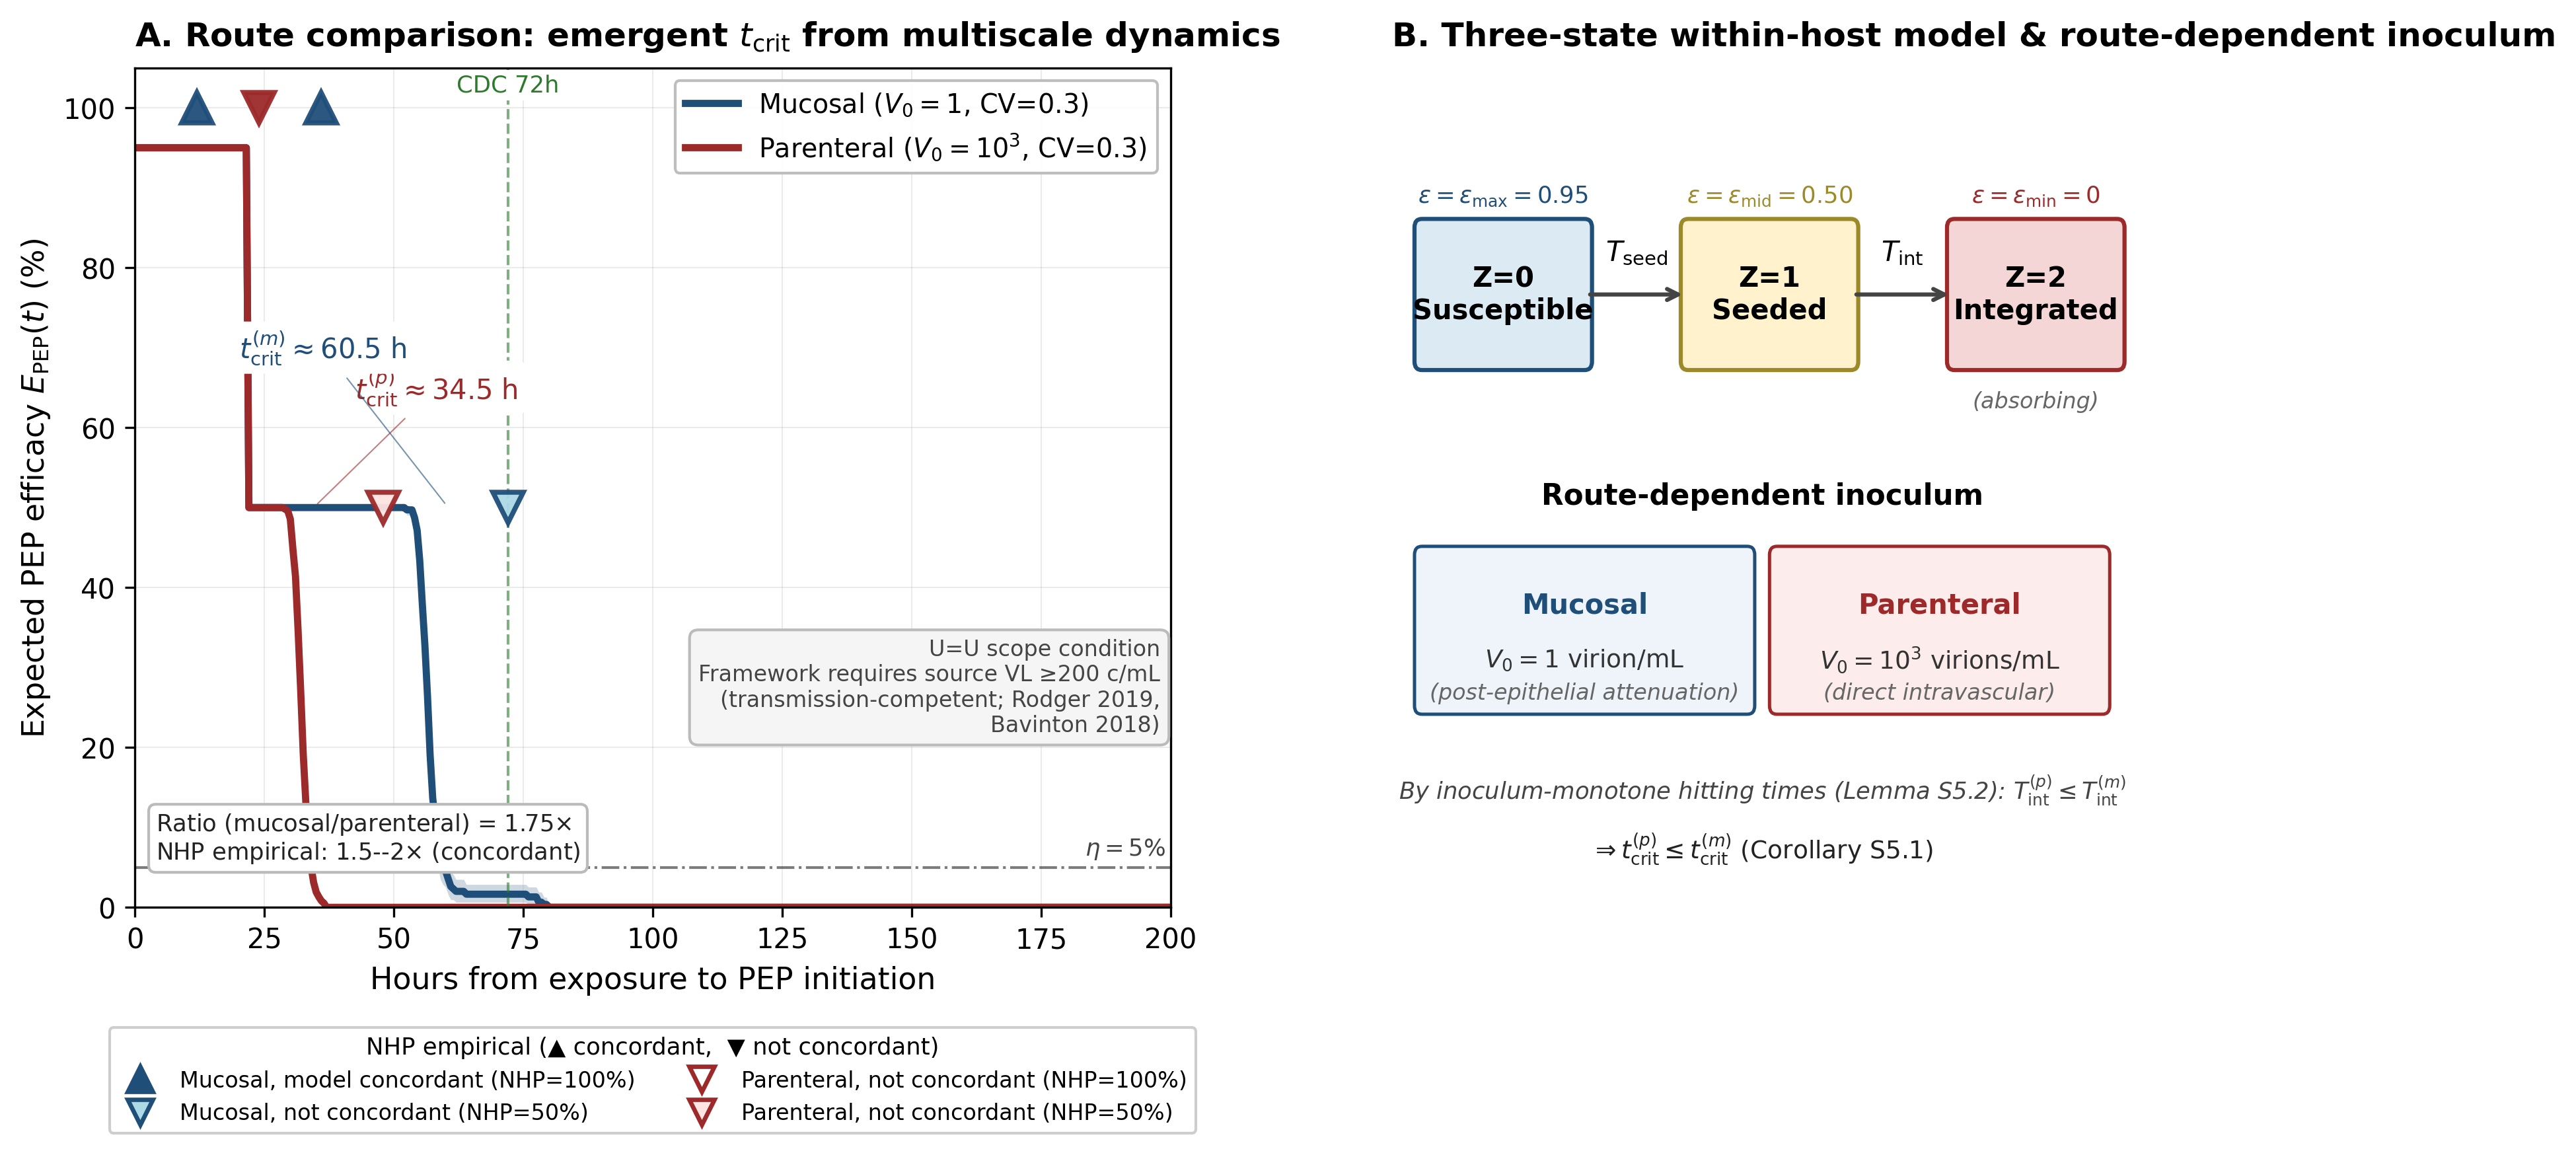
\includegraphics[width=\textwidth]{figures/Figure_1_Route_Dependent_PEP_Efficacy_Decay.png}
\caption{\textbf{Route-dependent PEP efficacy decay and prevention window compression.}
(\textbf{A}) Expected PEP efficacy $\Epep(t)$ as a function of hours post-exposure for mucosal (blue, $V_{0} = 1$) and parenteral (red, $V_{0} = 10^{3}$) routes, derived from the multiscale within-host model ($N = 500$ realizations per cell, CV $= 0.3$ on $\beta, c, \delta, \alpha$). Shaded bands: 95\% credible intervals from stochastic replications. Inset annotation marks U=U scoping (the framework applies only to transmission-competent exposures with source VL $\geq 200$ c/mL; per PARTNER2 / modern operational definition; see Methods). Dashed green vertical line: CDC 72-hour guideline. Dot-dash gray line: 5\% efficacy threshold ($\eta = 0.05$). Vertical dotted lines: verified $\tcrit$ values. Triangles: NHP protection data --- up-triangles concordant with model, down-triangles non-concordant. Parenteral $\tcrit \approx 34.5$~h ($V_{0} = 10^{3}$, CV $= 0.3$); mucosal $\tcrit \approx 60.5$~h ($V_{0} = 1$, CV $= 0.3$); compression ratio $\approx 1.75\times$ (concordant with NHP empirical 1.5--2$\times$ range).
(\textbf{B}) Schematic of the three-state within-host model and route-dependent inoculum. Parenteral inoculum ($10^{3}$ virions/mL) reaches integration threshold earlier than mucosal (1~virion/mL), establishing stochastic dominance in $\Tint$ by ODE monotone comparison.
Values reproducible from \texttt{Nyx-Dynamics/Prevention-Theorem} at commit \texttt{37e27ea} (\texttt{SRC/multiscale\_model/results\_v3/heterogeneity\_summary.csv}).}
\label{fig:route}
\end{figure}

\begin{figure}[H]
\centering
\includegraphics[width=\textwidth]{figures/Figure_2_Stochastic_Efficacy_VL_Uncertainty.png}
\caption{\textbf{Stochastic efficacy analysis under source VL uncertainty} (Monte Carlo extension, $N = 10{,}000$).
(\textbf{A}) Expected PEP efficacy (mean $\pm$ 50\% / 95\% CI bands) for four source VL distributions (PWID untreated: mean $\log_{10} = 4.5$; PWID mixed treatment: 3.2; general HIV+ community: 3.8; acute-infection-enriched: 5.0) over 0--120~h. Vertical reference lines: 24-h PEP initiation (purple dashed); 72-h CDC guideline (gray dashed). Horizontal reference at 50\% efficacy threshold. The framework applies to transmission-competent exposures only (source VL $\geq 200$ c/mL); U=U exposures are outside scope (Methods).
(\textbf{B}) Source VL probability densities on a $\log_{10}$ axis from LLoD ($\sim 20$ c/mL) to $10^{7}$ c/mL. \textbf{Vertical green dotted line at LLoQ $= 200$ c/mL} marks the U=U operational threshold (per PARTNER2; Rodger 2019; Bavinton 2018); below this VL, transmission risk is functionally zero and the framework is not applicable. Vertical orange dotted line at $10^{4}$ c/mL and red dotted line at $10^{5}$ c/mL mark inflection points used in the route-compression analysis. Panel B is the natural location for the U=U threshold marker; Panel A's hours-from-exposure axis precludes a literal VL-axis band.
(\textbf{C}) Probability of sub-therapeutic PEP, $P(\text{efficacy} < 50\%)$, by hours-from-exposure for each VL distribution. By 48~h, $P(<50\%) = 100\%$ across all distributions regardless of VL profile.
(\textbf{D}) VL knowledge premium --- the absolute gain in expected efficacy from knowing the source VL at PEP initiation versus marginalizing over the VL distribution --- for the two most clinically actionable distributions (PWID untreated; acute-infection-enriched network). Premium peaks within Regime~2 ($\sim$18--24~h) at 2.85--3.65 pp, where source VL testing is most decision-relevant.}
\label{fig:stochastic}
\end{figure}

\begin{figure}[H]
\centering

\includegraphics[width=\textwidth]{figures/Figure_3_City_Stratified_PEP_Efficacy.png}
\caption{\textbf{City-stratified PEP efficacy across 34 US metropolitan areas.}
(\textbf{A}) Expected PEP efficacy at city-specific structural delay for 34 cities (AIDSVu 2023), sorted by efficacy. Color: barrier category (green: low $<$8~h; orange: moderate 8--30~h; red: high $>$30~h).
(\textbf{B}) Structural delay vs.\ expected efficacy (Pearson $r = -0.935$); bubble size proportional to IDU prevalence. Labeled outliers: Hartford CT (24.4~h, highest structural delay, 23.4\% IDU); San Juan PR (13.3~h, highest community VL burden, 22.2\% IDU); Milwaukee WI (1.9~h, lowest barrier).
(\textbf{C}) Joint VL burden $\times$ structural delay risk surface; color encodes expected efficacy.
(\textbf{D}) Actual vs.\ 24-hour counterfactual efficacy by city. For 33/34 cities, actual efficacy exceeds counterfactual because structural delays are currently shorter than 24~h; Hartford is the exception. The 19.5~pp range across cities is almost entirely attributable to structural delay ($r = -0.935$) rather than community VL ($r = -0.084$). \textit{Scope notes:} (i) AIDSVu surveillance data are aggregated across sex; the city-stratified analysis pools across sex within AIDSVu categories (see Methods §Sex as a biological variable). (ii) AIDSVu late-diagnosis and viral suppression data are aggregated across mode of HIV acquisition and cannot be reliably subset to U=U status; this figure pools all source-VL strata in the surveillance denominator, consistent with the Methods specification of $\Faccess$.}
\label{fig:city}
\end{figure}

% =========================================================================
% Tables
% =========================================================================
\clearpage
\section*{Tables}

\begin{table}[H]
\centering
\caption{\textbf{NHP PEP timing data by route and per-timepoint model concordance.} Multiscale model output computed at the canonical operating point (CV $= 0.3$); see numerical claims summary CSV for reproducibility provenance.}
\label{tab:nhp}
\small
\begin{tabular}{@{}llllllc@{}}
\toprule
\textbf{Route} & \textbf{Study} & \textbf{Delay} & \textbf{NHP protection} & \textbf{Model $\Epep$} & \textbf{Per-timepoint} \\
\midrule
Parenteral (IV)   & Tsai 1998\cite{tsai1995}    & 24~h & 1.00 & 0.50 & not concordant \\
                  & Tsai 1998                   & 48~h & 0.50 & 0.00 & not concordant \\
Mucosal (vaginal) & Otten 2000\cite{otten2000}  & 12~h & 1.00 & 0.95 & concordant \\
                  & Otten 2000                  & 36~h & 1.00 & 0.95 & concordant \\
                  & Otten 2000                  & 72~h & 0.50 & 0.016 & not concordant \\
\bottomrule
\end{tabular}

\vspace{0.3em}
\footnotesize
\textbf{Compression-ratio concordance.} The model's mucosal/parenteral $\tcrit$ ratio at $\eta = 0.05$ is $60.5/34.5 = 1.75\times$, concordant with the empirical NHP range of $\sim$1.5--2$\times$ spanned by Tsai 1998 (parenteral half-protection at 48~h) and Otten 2000 (mucosal half-protection at 72~h: $72/48 = 1.50\times$). \textbf{Per-timepoint discordance.} The within-host kinetic model captures full protection at early Otten timepoints but under-predicts protection at the late Otten and both Tsai timepoints; we interpret this as evidence of NHP-specific protective contributions (innate immunity, eclipse-phase containment) not captured by the within-host kinetic framework alone. The compression result and the absolute-timepoint result are independent: the compression result is robust to the model's domain limitations.
\end{table}

\begin{table}[H]
\centering
\caption{\textbf{Stochastic efficacy metrics by VL distribution at key time points.}}
\label{tab:stochastic}
\small
\begin{tabular}{@{}lcccccc@{}}
\toprule
\textbf{Distribution} & \textbf{24~h mean} & \textbf{36~h mean} & \textbf{48~h $P(<50\%)$} & \textbf{48~h $P$(futile)} & \textbf{72~h $P$(futile)} & \textbf{Peak CI (time)} \\
\midrule
PWID untreated      & 65.5\% & 44.6\% & 100\% & 9.1\%  & 91.8\% & 39.7~pp (49~h) \\
PWID mixed Tx       & 75.4\% & 52.8\% & 100\% & 3.1\%  & 56.5\% & 40.1~pp (54~h) \\
General community   & 71.2\% & 49.2\% & 100\% & 3.5\%  & 76.0\% & 39.8~pp (54~h) \\
Acute-enriched      & 61.2\% & 41.3\% & 100\% & 13.8\% & 98.8\% & 37.4~pp (49~h) \\
\bottomrule
\end{tabular}

\vspace{0.3em}
\footnotesize
$P$(futile) $= P(\text{efficacy} < 5\%)$. CI~$=$~peak 95\% credible interval width in percentage points (pp). $P(<50\%) =$~probability that efficacy falls below majority protection. At 48~h, $P(<50\%) = 100\%$ across all distributions regardless of VL profile.
\end{table}

\begin{table}[H]
\centering
\caption{\textbf{$\Faccess \times \tcrit$ envelope sensitivity to parameterization} (Equation~\ref{eq:bound}, $\eta = 0.05$, $\emax = 0.95$, $\tcrit^{(p)} = 34.5$~h).}
\label{tab:bound}
\small
\begin{tabular}{@{}lcc@{}}
\toprule
\textbf{$\Faccess$ parameterization} & \textbf{$\Faccess(34.5\,\text{h})$} & \textbf{Envelope $\Ebarpep$ upper bound} \\
\midrule
Log-normal median 72~h, GSD 2.0 (JID-consistent)  & 0.121 & $\leq 15.9\%$ \\
Log-normal median 96~h, GSD 2.0 (canonical)       & 0.070 & $\leq 11.3\%$ \\
Log-normal median 110~h, GSD 2.0                  & 0.054 & $\leq 9.8\%$  \\
Log-normal median 120~h, GSD 2.0                  & 0.046 & $\leq 9.1\%$  \\
\bottomrule
\end{tabular}

\vspace{0.3em}
\footnotesize
\textbf{Reading the envelope.} The $\Faccess \times \tcrit$ bound is the most generous (envelope) reading of population-level PEP efficacy; cascade-based point estimates (Section: Population-level efficacy) yield 0.003--0.7\% under current US policy, one to four orders of magnitude below the envelope. The envelope is not the abstract's load-bearing claim; it is an analytical consistency check on the cascade-based central estimates. The qualitative ``below 10\%'' framing is supported by the cascade evidence; the envelope value depends on the modeling choice for $\Faccess$ median.
\end{table}

\end{document}
